\section{Prediction of cell organelles}
\subsection{Overfitting}

\begin{figure}[htb]
	\begin{center}
		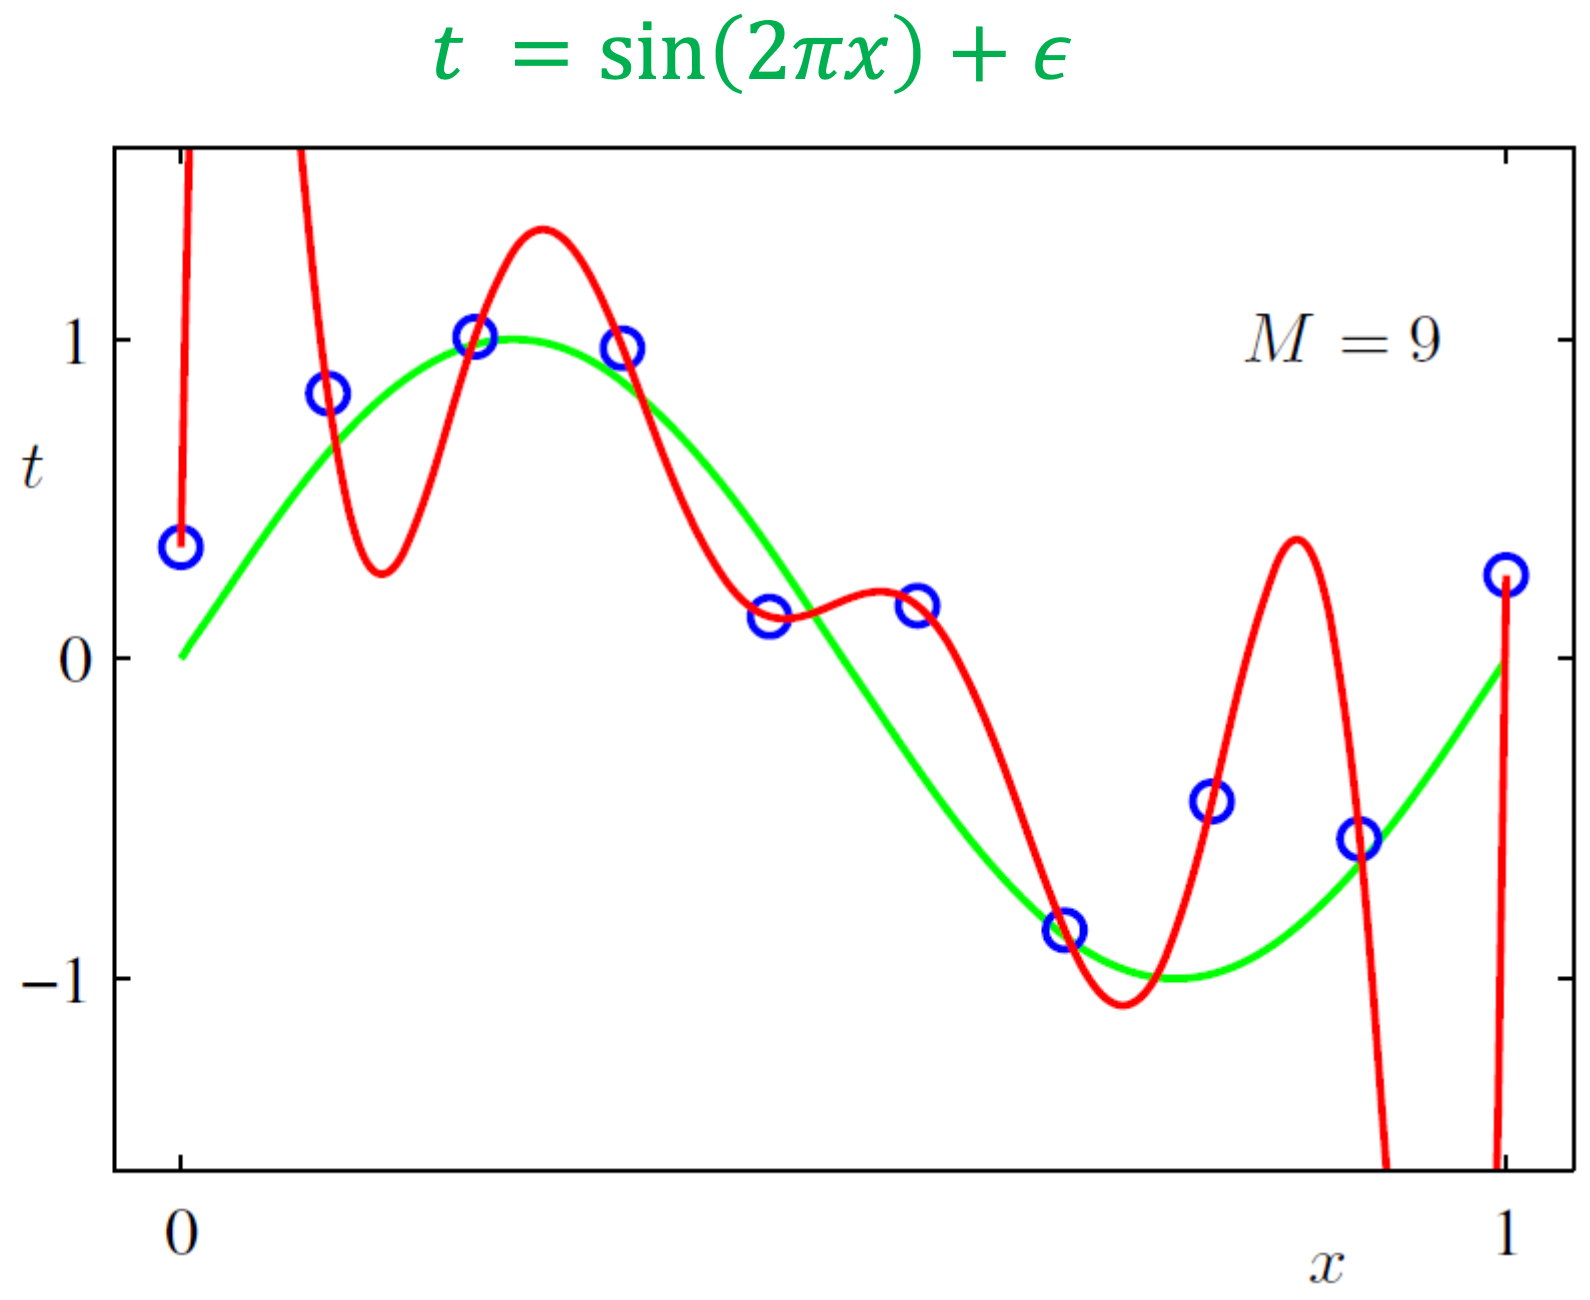
\includegraphics[width=0.6\linewidth]{bilder/overfit.png}
		\caption{Overfitting}\label{fig:overfit}
	\end{center}
\end{figure}

(Bishop book)

\subsubsection{Early-stopping}
\subsubsection{Regularization}
\begin{figure}[htb]
	\begin{center}
		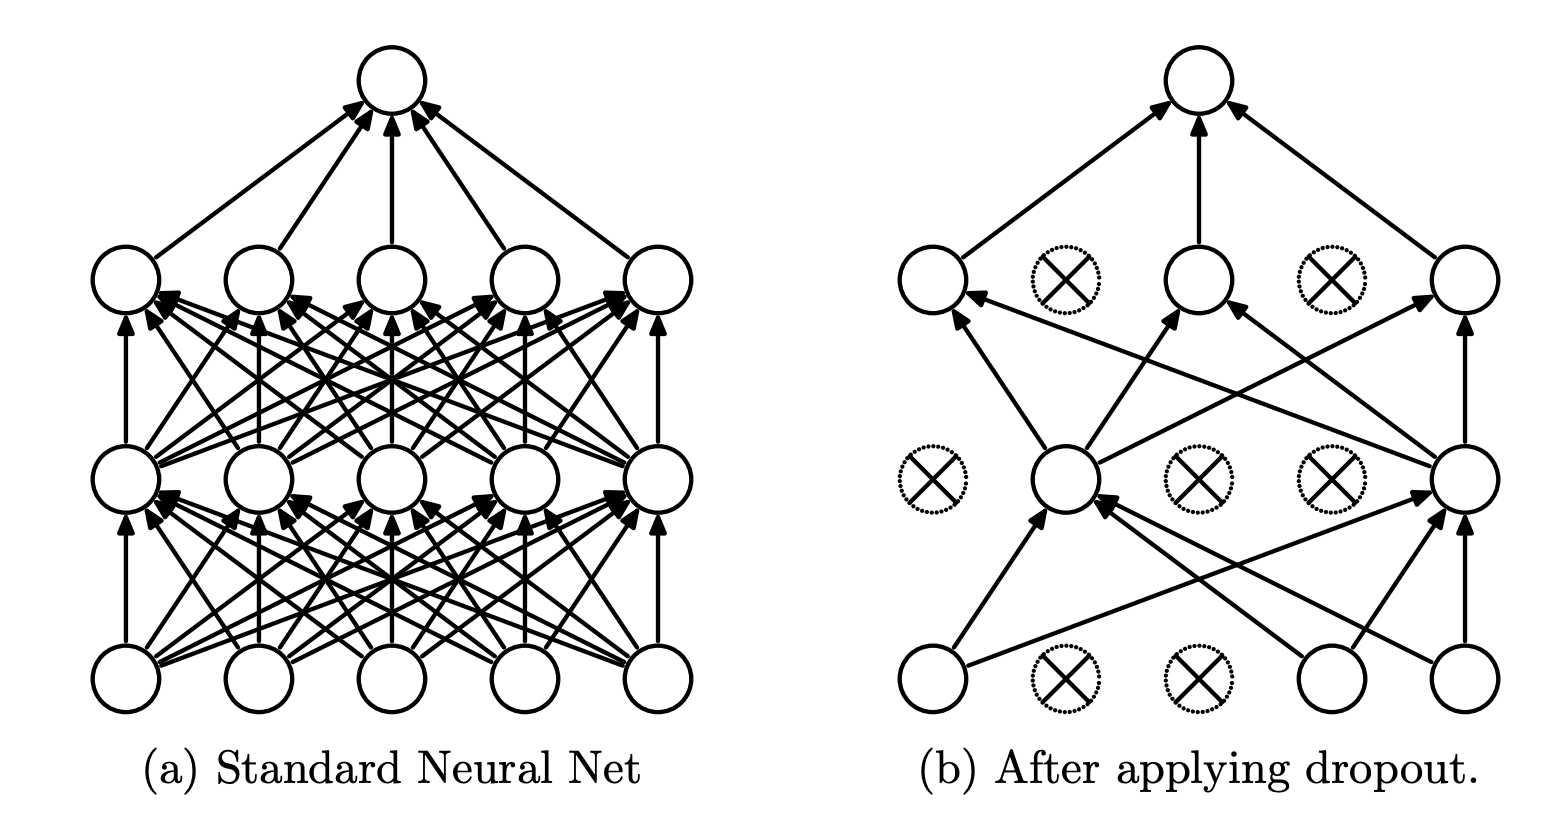
\includegraphics[width=0.8\linewidth]{bilder/dropout.png}
		\caption{Dropout}\label{fig:dropout}
	\end{center}
\end{figure}


\begin{figure}[htb]
    \centering
    \begin{minipage}{.5\textwidth}
      \centering
      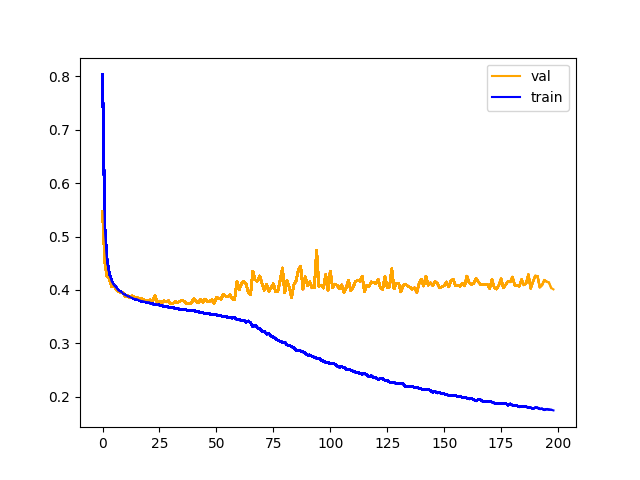
\includegraphics[width=\linewidth]{bilder/firt-train-overfit.png}
      \caption{Not regularized}
      \label{fig:first-train-overfit}
    \end{minipage}%
    \begin{minipage}{.5\textwidth}
      \centering
      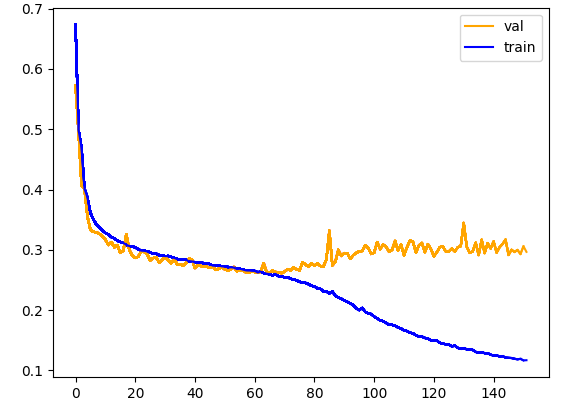
\includegraphics[width=\linewidth]{bilder/first-train-regularized.png}
      \caption{Regularized}
      \label{fig:first-train-regularized}
    \end{minipage}
\end{figure}

\subsubsection{Network reduction}
\subsubsection{Expansion of the training data}
